\begin{frame}
\frametitle{Machine Learning Review: What is Generalization Error?}

\vspace{-0.1in}
\begin{equation*}
    \text{generalization error} = |\text{test error} - \text{training error}|
\end{equation*}

\vspace{-0.3in}
\begin{center}
\resizebox{!}{2.5in}{
    \small
\begin{tikzpicture}
\node {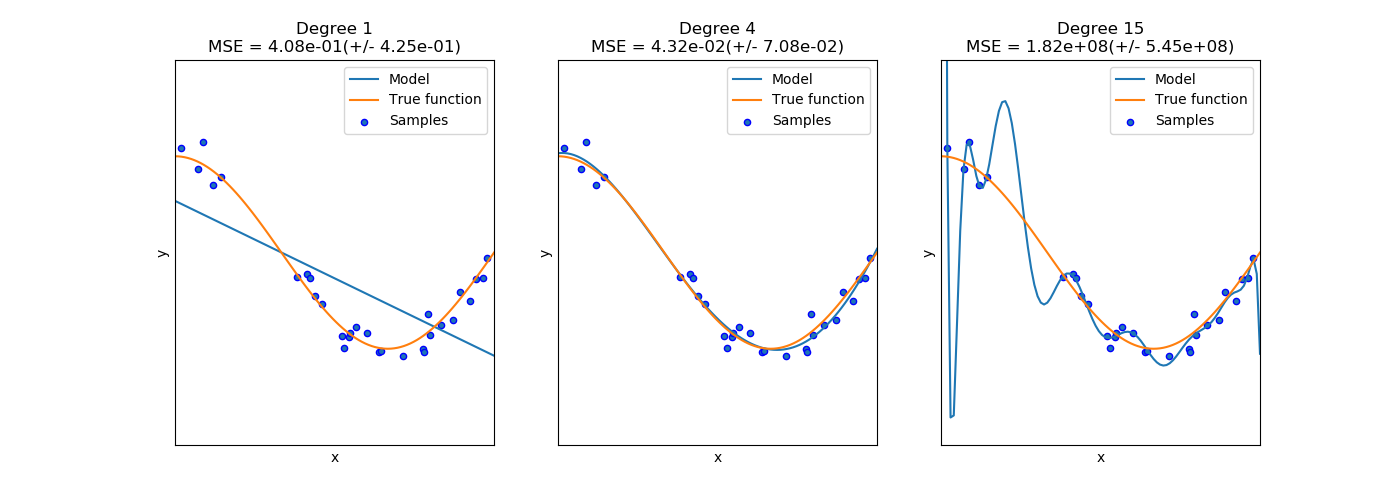
\includegraphics[height=2in,trim=100 0 0 0,clip]{img/over-under-fit}};

    \node at (-7.25,0) {};

    \uncover<2->{
    \draw[draw=red,line width=2pt] (-4.5,-2.5) -- (-3.95,-1.5);
    \node at (-4,-2.75) {\color{red}high training error / high test error};
    \node at (-4,-3.25) {\color{darkgreen} low generalization error};
    \node at (-4,-3.75) {\color{red}(underfit)};
}

    \uncover<3-> {
        \node at (3,-2.75) {\textcolor{darkgreen}{low training error} / \textcolor{red}{high test error}};
    \node at (3,-3.25) {\color{red}high generalization error};
    \node at (3,-3.75) {\color{red}(overfit)};

    \draw[draw=red,line width=2pt] (3.5,-2.5) -- (2.95,-1.5);
}

    \uncover<4-> {
    \node at (-0.5,3) {\color{darkgreen}low training error/low test error/low generalization error};
    \draw[draw=darkgreen,line width=2pt] (-0.5,2.5) -- (-1,1.5);
}

    \uncover<5>{
    \draw[->, line width=1.5pt,double distance=1pt] (-4.5,0.25) --(-1.5,0.25);
    \node at(-4,0.5) {better features};
}

    \uncover<6>{
    \draw[->, line width=1.5pt,double distance=1pt] (3.5,0.25) --(0.5,0.25);
    \node at(4,0.5) {\textbf{this talk}};
}
\end{tikzpicture}
}
\end{center}

    \vspace{-0.2in}
{
\fontsize{4}{4}
{\tiny Image source:} \url{https://scikit-learn.org/stable/auto_examples/model_selection/plot_underfitting_overfitting.html}
}
\end{frame}
